% четвертая часть

\section{Автоматизированный анализ данных}

Коммунальные компании постоянно сталкиваются с неучтенными расходами воды.
Чтобы справиться с утечками и сократить неучтенные расходы воды, необходимо четко представлять себе ситуацию в распределительной сети. \cite{smartcity}

Наличие нужных данных в нужное время значительно облегчает борьбу с потерей и неучтенными расходами воды и повышает эффективность этих действий. Автоматизированная система учета отображает реальное состояние распределительной сети, помогает выявить различные типы неучтенных расходов и сократить потери воды. 

Рассмотрим проблему, когда от счетчика не поступает импульс. Есть два варианта:
\begin{itemize}
	\item Проблемы с самим счетчиком, например зависает счетный механизм
	\item Проблемы с телеметрией, обрыв линии, короткое замыкание, не исправен геркон
\end{itemize}

Ошибка №1. Проблемы со счетчиком ХВС. 

Потребление ХВС = 0 за сутки, при этом потребление ГВС > 0 за сутки.

Алгоритм поиска:

Находим разность между показаниями счетчиков ХВС и ГВС, за текущее число и за вчерашнее.
Оставляем значения счетчиков ХВС и ГВС, где разность ХВС = 0.
Убираем значения счетчиков ХВС и ГВС, где разность ГВС = 0.

Оставшиеся счетчики ХВС являются проблемными (можно сравнивать не за сутки, а за 3 или 5).

Ошибка №2. Проблемы со счетчиком ГВС.

Потребление ГВС = 0 за неделю, при этом потребление ХВС > 0 за неделю.

Алгоритм поиска:

Находим разность между показаниями счетчиков ХВС и ГВС неделю назад и за текущее число.
Оставляем значения счетчиков ХВС и ГВС, где разность ГВС = 0.
Убираем значения счетчиков ХВС и ГВС, где разность ХВС = 0.

Получили счетчики, которые попадают в поле подозрения.
Нужно провести отбор, возможно горячей водой просто не пользуются.

Убираем счетчики, у которых значения ГВС < 5 и значение ХВС < 10.
Оставшиеся счетчики ГВС являются проблемными и требуют ручной проверки.

Ошибка №3. Проблемы со счетчиком ХВС и ГВС.

Потребление ХВС = 0, ГВС = 0 за неделю, при этом потребление Э  >= Ср.Ар. за предыдущую неделю.

Алгоритм поиска:

Находим разность между показаниями счетчиков ХВС и ГВС неделю назад и за текущее число.
Оставляем значения счетчиков ХВС и ГВС, где разность ГВС = 0 и ХВС = 0.
Находим среднее арифметическое потребление электричества за предыдущую неделю.
Если потребление электроэнергии за неделю больше чем среднее арифметическое значение, то счетчики попадают в список проблемных счетчиков.

Ошибка №4. Проблемы с электросчетчиком.

Потребление Электричества = 0 за сутки, при этом потребление ХВС > 0 и/или ГВС > 0 за сутки и более.

\subsection{Анализ показаний приборов учета}

Учет и анализ коммунальных ресурсов дает возможность выявить их перерасход, вызванный, возможно, и халатным отношением, либо неисправностью приборов учета. Также становится прозрачным перерасход ресурсов и несанкционированное их потребление.\cite{journal}

«Личный кабинет» программы СКАУТ позволяет получить часовые, суточные и ежемесячные данные в виде таблиц и графиков, что позволяет удобно анализировать расход ресурсов.

Детализация данных для всестороннего анализа.
Посуточная статистика. Пример приведен на рис.~\ref{fig:day}
\begin{figure}[H]
	\centering
	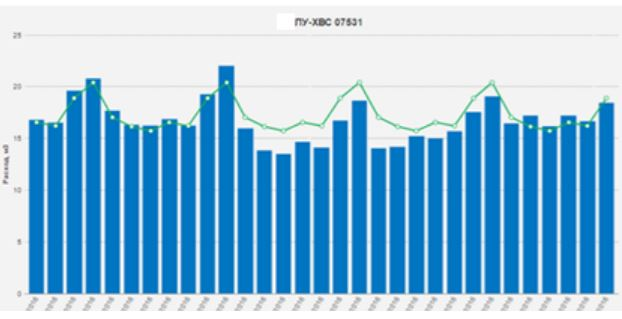
\includegraphics[width=0.7\linewidth]{pics/day}
	\caption{Посуточное потребление}
	\label{fig:day} 
\end{figure}
Почасовая статистика. Пример приведен на рис.~\ref{fig:hour}
\begin{figure}[H]
	\centering
	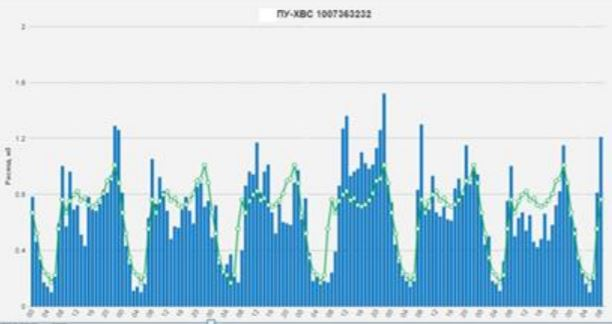
\includegraphics[width=0.7\linewidth]{pics/hour}
	\caption{Почасовые показания}
	\label{fig:hour} 
\end{figure}

С выведением информации по средне статическому потреблению.
Графическое представление, особенно за длительные сроки, даёт наглядную картину работы водосчетчиков и электросчетчиков. 

Несколько сложнее обнаруживать утечки в системе горячего водоснабжения. Непрерывный и неравномерный разбор горячей воды затрудняет их определение. Использование статистики потребления горячей воды жилым домом в ночные часы (3 часа ночи) позволяет улавливать фоновые потери для каждого дома. В основном это передавливание горячей воды в трубопровод холодного водоснабжения через неисправные квартирные смесители. Установив для каждого дома фоновый уровень потерь, можно контролировать появление протечек. До настоящего времени нами не было обнаружено таких протечек, однако данным методом в Обнинске были выявлены два 100 квартирных дома, где фоновое потребление холодной воды на дом достигало 600 литров в час и более. В квартирах одного их них были обнаружены два неисправных сливных бачка, в другом доме протекал вентиль в подвале, и вода уходила в ливневую канализацию. После ремонтов фоновое потребление в этих домах установилось на уровне 250–300 литров в час. \cite{journal2}

Так же известно, что потребление горячей воды не может превышать потребление холодной. Данная проблема сигнализирует нам об неисправности счетчика. С помощью наложения двух графиков потребления горячей и холодной воды, можем наглядно увидеть проблемные счетчики.